\section{AI 기반 수학 문제 자동 채점 시스템 개발}

\subsection{프로젝트 시작과 준비 과정}

\begin{figure}[H]
    \centering
    \includegraphics[width=0.8\textwidth]{images/1_math_initial_planning.png}
    \caption{초기 프로젝트 기획 과정}
    \label{fig:math_initial_planning}
\end{figure}

전남과학고 수학 지필평가를 치른 이후 수업시간, 선생님께서 하신 말씀이 계기가 되었습니다. 한 친구가 시험 점수가 언제 나오냐고 질문했을 때, 선생님께서는 80여 명의 시험지를 혼자 채점하려면 적어도 일주일은 걸릴 것 같다고 하셨습니다. 모든 문제가 주관식·서술형인 학교 수학 시험의 특성상 채점에 오랫동안 공을 들여야 하고, 오류 가능성도 높았습니다. 그때, ``이건 AI로 해결할 수 있을 것 같은데?''라는 생각에서 프로젝트가 시작되었습니다.

처음에는 단순히 OCR(광학 문자 인식)을 활용해 답만 확인하는 시스템을 생각했습니다. 하지만 단순히 정답여부만 알기보다는 학생들의 풀이 과정을 이해하고 부분 점수를 부여하는 것이 더 중요하다는 것을 알게 되었습니다.

\subsection{도전과 시행착오}

\subsubsection{전통적 OCR 접근}

\begin{figure}[H]
    \centering
    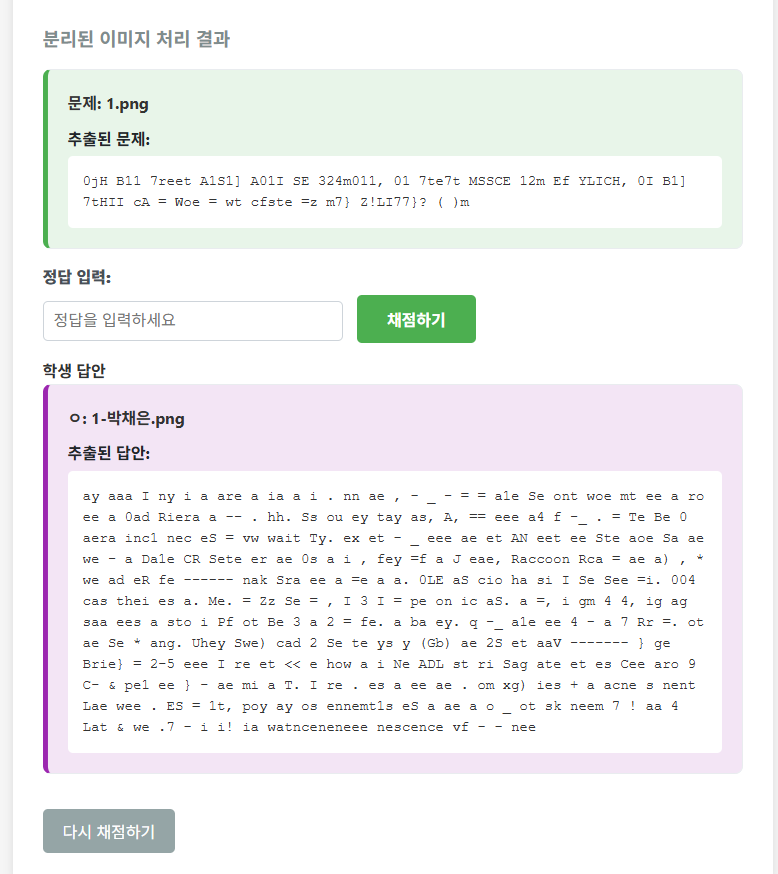
\includegraphics[width=0.5\textwidth]{1/image02.png}
    \caption{OCR 방식의 한계 - 수식 인식 실패 사례}
    \label{fig:math_ocr_failure}
\end{figure}

처음에는 Python의 pytesseract 라이브러리를 사용해 손글씨를 텍스트로 변환하려 했습니다. `kor+eng' 언어 설정으로 OCR을 수행했지만, 수학 기호와 복잡한 수식, 필체 다양성으로 인해 인식률이 매우 낮았습니다. 특히 분수나 제곱근 같은 수학 기호는 거의 인식하지 못했습니다.

{컴퓨터 비전 모델}

\begin{figure}[H]
    \centering
    \includegraphics[width=0.8\textwidth]{images/1_math_cv_attempt.png}
    \caption{컴퓨터 비전 모델 훈련 시도}
    \label{fig:math_cv_attempt}
\end{figure}

다음으로 YOLO와 같은 객체 탐지 모델을 훈련시켜 수식을 인식하려 했습니다. 하지만 충분한 훈련 데이터를 구하기 어려웠고, 모델이 수식의 의미를 이해하지 못해 채점에는 활용할 수 없었습니다.

\subsubsection{세 번째 시도: LLM Vision API 활용}

\begin{figure}[H]
    \centering
    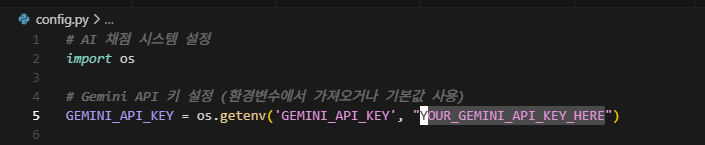
\includegraphics[width=0.48\textwidth]{1/image01.png}
    \caption{Gemini API 적용}
    \label{fig:math_gemini_application}
\end{figure}
\begin{figure}[H]
    \centering
    \includegraphics[width=0.8\textwidth]{images/1_math_gemini_success.png}
    \caption{Gemini Vision API를 활용한 성공적인 채점}
    \label{fig:math_gemini_success}
\end{figure}

Google Gemini Vision API를 발견한 것은 전환점이었습니다. google.generativeai 라이브러리를 통해 이미지를 직접 분석할 수 있었고, 수학적 맥락까지 파악할 수 있었습니다. GeminiModel 클래스를 만들어 API를 체계적으로 관리했습니다.

\subsection{프롬프트 엔지니어링의 중요성}

\begin{figure}[H]
    \centering
    \includegraphics[width=0.8\textwidth]{images/1_math_prompt_evolution.png}
    \caption{프롬프트 개선 과정}
    \label{fig:math_prompt_evolution}
\end{figure}

단순히 `이 수학 문제를 채점해줘'라는 프롬프트로는 일관성 있는 결과를 얻을 수 없었습니다. 수십 번의 실험 끝에 다음과 같은 구조화된 프롬프트를 개발했습니다.

\paragraph{최종 채점 프롬프트 구조.}\smallskip
\begin{lstlisting}[language=Python, basicstyle=\footnotesize\ttfamily]
ENHANCED_SYSTEM_PROMPT = """
You are a math teacher grading students' math problem solutions.

**Grading Distribution (Total 10 points):**
- Process Score: 6 points (3 items)
  - Problem understanding and approach: 2 points
  - Logical consistency of solution: 2 points
  - Calculation and expression accuracy: 2 points
- Answer Score: 4 points
  - Full 4 points if final answer is completely accurate
  - Fractions must match exactly (5/6 != 6/5)

**JSON Format Output:** 
{
  "detected_info": {
    "student_name": "Student name or 'Not detected'",
    "problem_number": "Problem number or 'Not detected'"
  },
  "grading_result": {...},
  "feedback": "Specific improvement suggestions"
}
"""
\end{lstlisting}

\subsection{시스템 아키텍처 구현: 프론트엔드와 백엔드 통합}

\begin{figure}[H]
    \centering
    \includegraphics[width=0.8\textwidth]{images/1_math_system_architecture.png}
    \caption{최종 시스템 아키텍처}
    \label{fig:math_system_architecture}
\end{figure}

\subsubsection{배치 처리 시스템}

대량의 답안을 효율적으로 처리하기 위해 비동기 배치 처리 시스템을 구현했습니다

Server-Sent Events(SSE)로 진행 상황을 실시간으로 표시함과 동시에 최대 5개 작업을 병렬 처리했습니다. 진행이 중단되면 중간 결과를 자동 저장해 즉시 복구하도록 했습니다.

\begin{figure}[H]
    \centering
    \includegraphics[width=0.8\textwidth]{images/1_math_batch_processing.png}
    \caption{배치 처리 진행 화면}
    \label{fig:math_batch_processing}
\end{figure}

\subsubsection{지능형 페이지 분석}

\begin{figure}[H]
    \centering
    \includegraphics[width=0.8\textwidth]{images/1_math_page_detection.png}
    \caption{다양한 답안 레이아웃 자동 감지}
    \label{fig:math_page_detection}
\end{figure}

학생들이 제출하는 답안의 형태는 매우 다양합니다. HTML/CSS/JavaScript로 구현한 웹 프론트엔드에서 PDF와 이미지 파일을 업로드하면, Python의 pdf\_processor.py가 페이지를 분할하고 page\_analyzer.py가 Gemini Flash API로 페이지 구조를 자동 분석합니다. 문제 번호와 학생 이름을 JSON 형식으로 추출하여 가로와 세로 레이아웃을 안정적으로 인식했습니다.

\subsection{실제 적용과 결과}

\begin{figure}[H]
    \centering
    \includegraphics[width=0.8\textwidth]{images/1_math_real_example.png}
    \caption{실제 학생 답안 채점 예시}
    \label{fig:math_real_example}
\end{figure}

\subsubsection{정량적 성과}

채점 시간이 크게 단축되고 일관성이 향상되었으며, 더 많은 학생들의 답안을 처리할 수 있게 되었습니다.

\begin{figure}[H]
    \centering
    \includegraphics[width=0.8\textwidth]{images/1_math_performance_metrics.png}
    \caption{성능 지표 대시보드}
    \label{fig:math_performance_metrics}
\end{figure}

\subsubsection{교육적 효과}

\begin{figure}[H]
    \centering
    \includegraphics[width=0.8\textwidth]{images/1_math_educational_impact.png}
    \caption{학생 성적 향상 추이}
    \label{fig:math_educational_impact}
\end{figure}

교사들이 채점에 소요하는 시간이 감소하여 개별 지도에 더 많은 시간을 할애할 수 있게 되었습니다. 개인별 약점 분석 리포트를 통해 맞춤형 학습이 가능해졌습니다.

\subsection{기술적 난제 해결 과정}

\subsubsection{멀티모달 아키텍처 구현}

프로젝트의 가장 큰 성과는 프론트엔드와 백엔드를 효과적으로 통합한 풀스택 시스템 구현입니다:

\begin{itemize}[leftmargin=*]
    \item \textbf{프론트엔드 (HTML/CSS/JavaScript)}: Drag\&Drop 파일 업로드, 실시간 프리뷰, 배치 처리 진행 표시
    \item \textbf{백엔드 (Python)}: 
    \begin{itemize}
        \item GradingService: Gemini Vision API 통합 및 채점 로직
        \item OcrService: pytesseract 기반 텍스트 추출 (폴백 옵션)
        \item PDFProcessor: PyPDF2로 다중 페이지 PDF 처리
        \item ImageService: PIL을 활용한 이미지 전처리
    \end{itemize}
    \item \textbf{API 통신}: RESTful API 설계, JSON 기반 데이터 교환
\end{itemize}

\subsubsection{정확도 향상을 위한 프롬프트 최적화}

120개 이상의 실제 답안으로 테스트하면서 프롬프트를 지속적으로 개선했습니다. 특히 ``5/6과 6/5는 다른 답''이라는 엄격한 기준을 적용하여 채점의 신뢰성을 높였습니다. 학년별(초등/중등/고등) 평가 기준을 차별화하여 맥락에 맞는 채점이 가능하도록 했습니다.

\subsubsection{API 제한 극복}

\begin{figure}[H]
    \centering
    \includegraphics[width=0.8\textwidth]{images/1_math_api_optimization.png}
    \caption{API 최적화 전략}
    \label{fig:math_api_optimization}
\end{figure}

Gemini API의 요청 제한과 이미지 크기 제한을 극복하기 위해 적응형 이미지 압축 알고리즘을 개발했습니다. 다중 API 키를 로테이션하고 지능형 캐싱으로 중복 요청을 최소화했습니다.

\subsubsection{오류 처리와 안정성}

\begin{figure}[H]
    \centering
    \includegraphics[width=0.8\textwidth]{images/1_math_error_handling.png}
    \caption{강건한 오류 처리 시스템}
    \label{fig:math_error_handling}
\end{figure}

AI 응답의 불확실성을 처리하기 위해 JSON 파싱 실패 시 자동 복구했습니다. 안전 필터가 트리거되면 재시도했고 타임아웃이 발생하면 폴백 처리로 안정성을 확보했습니다.